\documentclass[10pt,a4paper]{article}

\usepackage[utf8]{inputenc}		% Configuro la codificación
\input{config.tex}				% Archivo con los comandos globales como Título y autores
\input{preamble.tex}
\input{aux_functions.tex}		% Se proveen un conjunto de funciones extras

% Defino el path de los includegraphics
\graphicspath{{./Figuras/}}		% Directorio que contiene los graficos

% Defino el path para los input de .tex y de .eps
\makeatletter
\def\input@path{{./Figuras/}{./Secciones/}{./Cover_page/}}
\makeatother

% Defino el path del listings
\ifListings
%% Cambiar el nombre de la carpeta si se utilizan Listings
	\lstinputpath{{../Octave/}}
\fi

\definecolor{myred}{rgb}{0.5,0,0}
\definecolor{mygreen}{rgb}{0,0.5,0}



\begin{document}
		% Carátula (formal o simple,_formal o _simple respectivamente) con Resumen
		% incluido e Índice (si es necesario configurar en config.tex) del informe
		\input{cover_simple.tex}
	\setcounter{page}{1}

	\section{Enunciado}\label{sec:enunciado}
		
	Se considera un vehículo que se desplaza definiendo una trayectoria tal que la posición en cada instante resulta $\vect{p}(t)$, con una velocidad $\vect{v}(t)$ y una aceleración $\vect{a}(t)$, definidas en un plano de coordenadas $[x,y]$ de acuerdo a:
	\begin{equation*}
		\vect{p}(t) = \begin{bmatrix} p_x(t) \\[0.3em] p_y(t) \end{bmatrix} \qquad%
		\vect{v}(t) = \begin{bmatrix} v_x(t) \\[0.3em] v_y(t) \end{bmatrix} \qquad%
		\vect{a}(t) = \begin{bmatrix} a_x(t) \\[0.3em] a_y(t) \end{bmatrix}% 
	\end{equation*}

	Suponiendo que la dinámica de movimiento satisface las siguientes ecuaciones:
	\begin{equation}
		\begin{cases}
			\vect{\dot{p}}(t) = \vect{v}(t)\\
			\vect{\dot{v}}(t) = \vect{a}(t)\\
			\vect{\dot{a}}(t) = 0
		\end{cases}
		\label{eq:dinamica_enun}
	\end{equation}



	\section{Ejercicio 1}\label{sec:ej1}
		\subsection{Inciso a}
	Se define la variable de estado asociada a las ecuaciones de movimiento continuo como:
		\begin{equation*}
			\vect{x}(t) = \begin{bmatrix} \vect{p}(t) \\[0.3em] \vect{v}(t) \\[0.3em] \vect{a}(t) \end{bmatrix} \qquad%
			\dot{\vect{x}}(t) = \begin{bmatrix} \dot{\vect{p}}(t) \\[0.3em] \dot{\vect{v}}(t) \\[0.3em] \dot{\vect{a}}(t) \end{bmatrix}
		\end{equation*}

	Así el modelo resulta:
		\begin{equation*}
			\Sigma:
			\begin{cases}
				\dvect{x}(t) = A\: \vect{x}(t) + B \: \vect{\xi}(t) \\
				\vect{y}(t) = C\: \vect{x}(t) + \vect{\eta}(t)
			\end{cases}
		\end{equation*}
	donde $\vect{\xi}(t)$ es el ruido de proceso y $\vect{\eta}(t)$ el ruido de medición. La matriz $A$ contiene la información de la dinámica del sistema, $B$ es la matriz de entrada del ruido de proceso, y la matriz de salida es $C$, que conecta los estados con las mediciones. En la Figura \ref{fig:bloques} puede verse el diagrama en bloques del modelo.
	\graficarEPS{0.6}{bloques}{Diagrama en bloques del modelo.}{fig:bloques}
	
	Para poder tratar el sistema en forma digital, es necesario definir un período de muestreo $T$, que en este caso es igual a la unidad. De esta forma el modelo en tiempo discreto es el siguiente:
	
		\begin{equation*}
			\Sigma_{d}:
			\begin{cases}
				\vect{x}_{n + 1} = A_{d}\: \vect{x}_{n} + B_{d} \: \vect{\xi}_{n} \\
				\vect{y}_{n} = C_{d}\: \vect{x}_{n} + \vect{\eta}_{n}
			\end{cases}
		\end{equation*}
		
	donde ahora se obtienen nuevas matrices para el caso discreto. En dicho caso, a partir de las ecuaciones de la cinemática, se deduce que la matriz de la dinámica del sistema es:

		\begin{equation*}
			A_{d} = \begin{bmatrix} I & IT & I\frac{T^2}{2} \\[0.3em] 0 & I & IT \\[0.3em] 0 & 0 & I \end{bmatrix}
		\end{equation*}

	La matriz de salida $C_{d}$ dependerá de lo que se esté midiendo. Por ejemplo para el caso en que se sensen todas las variables será:
	
		\begin{equation*}
			C_{d} = \begin{bmatrix} I & 0 & 0 \\[0.3em] 0 & I & 0 \\[0.3em] 0 & 0 & I \end{bmatrix}
		\end{equation*}
		
		Para el caso en que alguna de las variables no se esté midiendo, será necesario eliminar alguna de las tres filas (de $2\times2$) de la matriz. En concreto se omite la primera, segunda o tercera fila, dependiendo si no se sensase posicion, velocidad o aceleración respectivamente. 
		En este modelo, la matriz $B$ se toma como la matriz identidad.
	En cuanto a los ruidos, se hace la suposición que se tratan de ruidos blancos con matrices de covarianza $Q_{d}$ para el ruido de proceso y $R_{d}$ para el ruido de medición. Cabe aclarar que el hecho de que se trate de ruidos blancos no implica que $Q_{d}$ y $R_{d}$ sean diagonales. Ambas matrices dan información de la correlación componente a componente de los vectores de ruido.
	
\subsection{Inciso b}

	El siguiente bloque de código contiene la definición de las matrices $A_{d}$ y $Q_{d}$.

	\begin{lstlisting}
	
config_m;			

datos_str = load('datos.mat');

Acel = datos_str.Acel;
Tiempo = datos_str.tiempo;
Pos = datos_str.Pos;
Vel = datos_str.Vel;

dim = 2;			% Se considera sólo x e y
tipos_variables = 3;		% Posición, Velocidad, Aceleración
cant_mediciones = length(Pos);
cant_estados = tipos_variables * dim;

% Datos
var_xip = 3e-4;
var_xiv = 2e-3;
var_xia = 1e-2;

%%%
T = 1;					% Suponiendo equiespaciado

% Variable de estado X = [P;V;A]
I = eye(dim);
Ad =[I		I*T	(T^2)/2*I;
     I*0	I	T*I;
     I*0	I*0	I];

% Covarianza del ruido de proceso
Qd = diag([ones(1,dim)*var_xip, ones(1,dim)*var_xiv, ones(1,dim)*var_xia]);

	\end{lstlisting}
	
% $Q_d=\begin{bmatrix} \sigma^2_{\xi_{px}} &&&&&\\[0.3em] &\sigma^2_{\xi_{py}}&&&&\\[0.3em] &&\sigma^2_{\xi_{vx}}&&&\\[0.3em] &&&\sigma^2_{\xi_{vy}}&&\\[0.3em] &&&&\sigma^2_{\xi_{ax}}&\\[0.3em] &&&&&\sigma^2_{\xi_{ay}}\end{bmatrix}$






	
		

		
	\section{Ejercicio 2}\label{sec:ej2}
		
	\begin{lstlisting}[caption=Script para la resolución del ejercicio 2]
%%%%%%%%%%%%%%%%%%%%%%%%%%%%%%%%%%
% EJERCICIO 2
%%%%%%%%%%%%%%%%%%%%%%%%%%%%%%%%%%
bool_p = 1;	% Inciso a
bool_v = 0;	% Inciso b
bool_a = 0;	% Inciso c


x0 = [40 -200 0 0 0 0]';
P0_0 = diag([100^2 100^2, 1 1, 0.1 0.1]);

%%%%% y_k = [I 0 0] [pk vk ak]' + ruido \eta
sigma_etap = 60;
sigma_etav = 2;
sigma_etaa = 0.1;


C = [eye(dim)*bool_p eye(dim)*bool_v eye(dim)*bool_a];

yk = C * ([Pos(:,1:dim) Vel(:,1:dim) Acel(:,1:dim)])' + randn(dim,cant_mediciones)*sigma_etap;
yk = yk'; % Así tiene la forma de Pos

R = eye(dim)*sigma_etap^2;
Bk1 = eye(cant_estados);


%%% ALGORITMO %%%%
xk1_k1 = x0;
Pk1_k1 = P0_0;
x = x0;
P = P0_0;
g = yk(1,:)';

for i=1:cant_mediciones-1
	% Predicción
	xk_k1 = Ad * xk1_k1;
	Pk_k1 =	Ad * Pk1_k1 * Ad' + Bk1 * Qd * Bk1.';
	gk = [innovaciones(yk(i,:),C,xk_k1)];

	% Corrección
	Kk = Pk_k1 * C'*(R + C*Pk_k1*C')^-1;
	xk_k = xk_k1 + Kk*(yk(i,:)' - C*xk_k1);
	Pk_k = (eye(dim*3) - Kk*C) * Pk_k1;
	
% PARA HACER SIMETRICA P, ALEJANDOSE DEL VALOR VERDADERO	
%		% Para hacerlo simétrico
%		for i=1:2
%			Pk_k=(Pk_k+Pk_k')/2;
%		end

	% Actualización
	xk1_k1 = xk_k;
	Pk1_k1 = Pk_k;


	% Guardo
	g = [g gk];
	x = [x xk_k];
	P = [P; Pk_k];
end

	\end{lstlisting}


	\section{Ejercicio 3}\label{sec:ej3}
		
	En el punto anterior se describió el algoritmo de Kalman. En el mismo hay una fase de inicialización de la estimación. En esta Sección se analizan las variaciones que se presentan a la hora de cambiar los valores iniciales. Por ejemplo se podría inicializar en un valor coincidente con los datos, con una varianza pequeña, en cuyo caso la estimación convergerá más rápido. Otro caso extremo es cuando el valor inicial es incorrecto, también con varianza pequeña, resultando en una convergencia mucho más lenta. La idea de este punto es la exploración de las distintas variantes de este tema y en cada caso se presentarán gráficos de la estimación de la trayectoria, de evolución de los errores y de la autocorrelación de las innovaciones.
	
	\subsection{Caso 1 - $\vect{x}_{0/0} = [40\;-200\;0\;0\;0\;0]^T$, $P^{'}_{0/0}=100\; P_{0|0}$} \label{sec:ej3a}
	
		Para el primer caso, se tiene un error en la estimación del estado inicial pequeño, pero una varianza grande. En este caso el algoritmo convergerá rápidamente a la trayectoria real. El resultado puede verse en la Figura \ref{fig:ej3a}.
	
		\begin{figure}[H]
			\centering
			%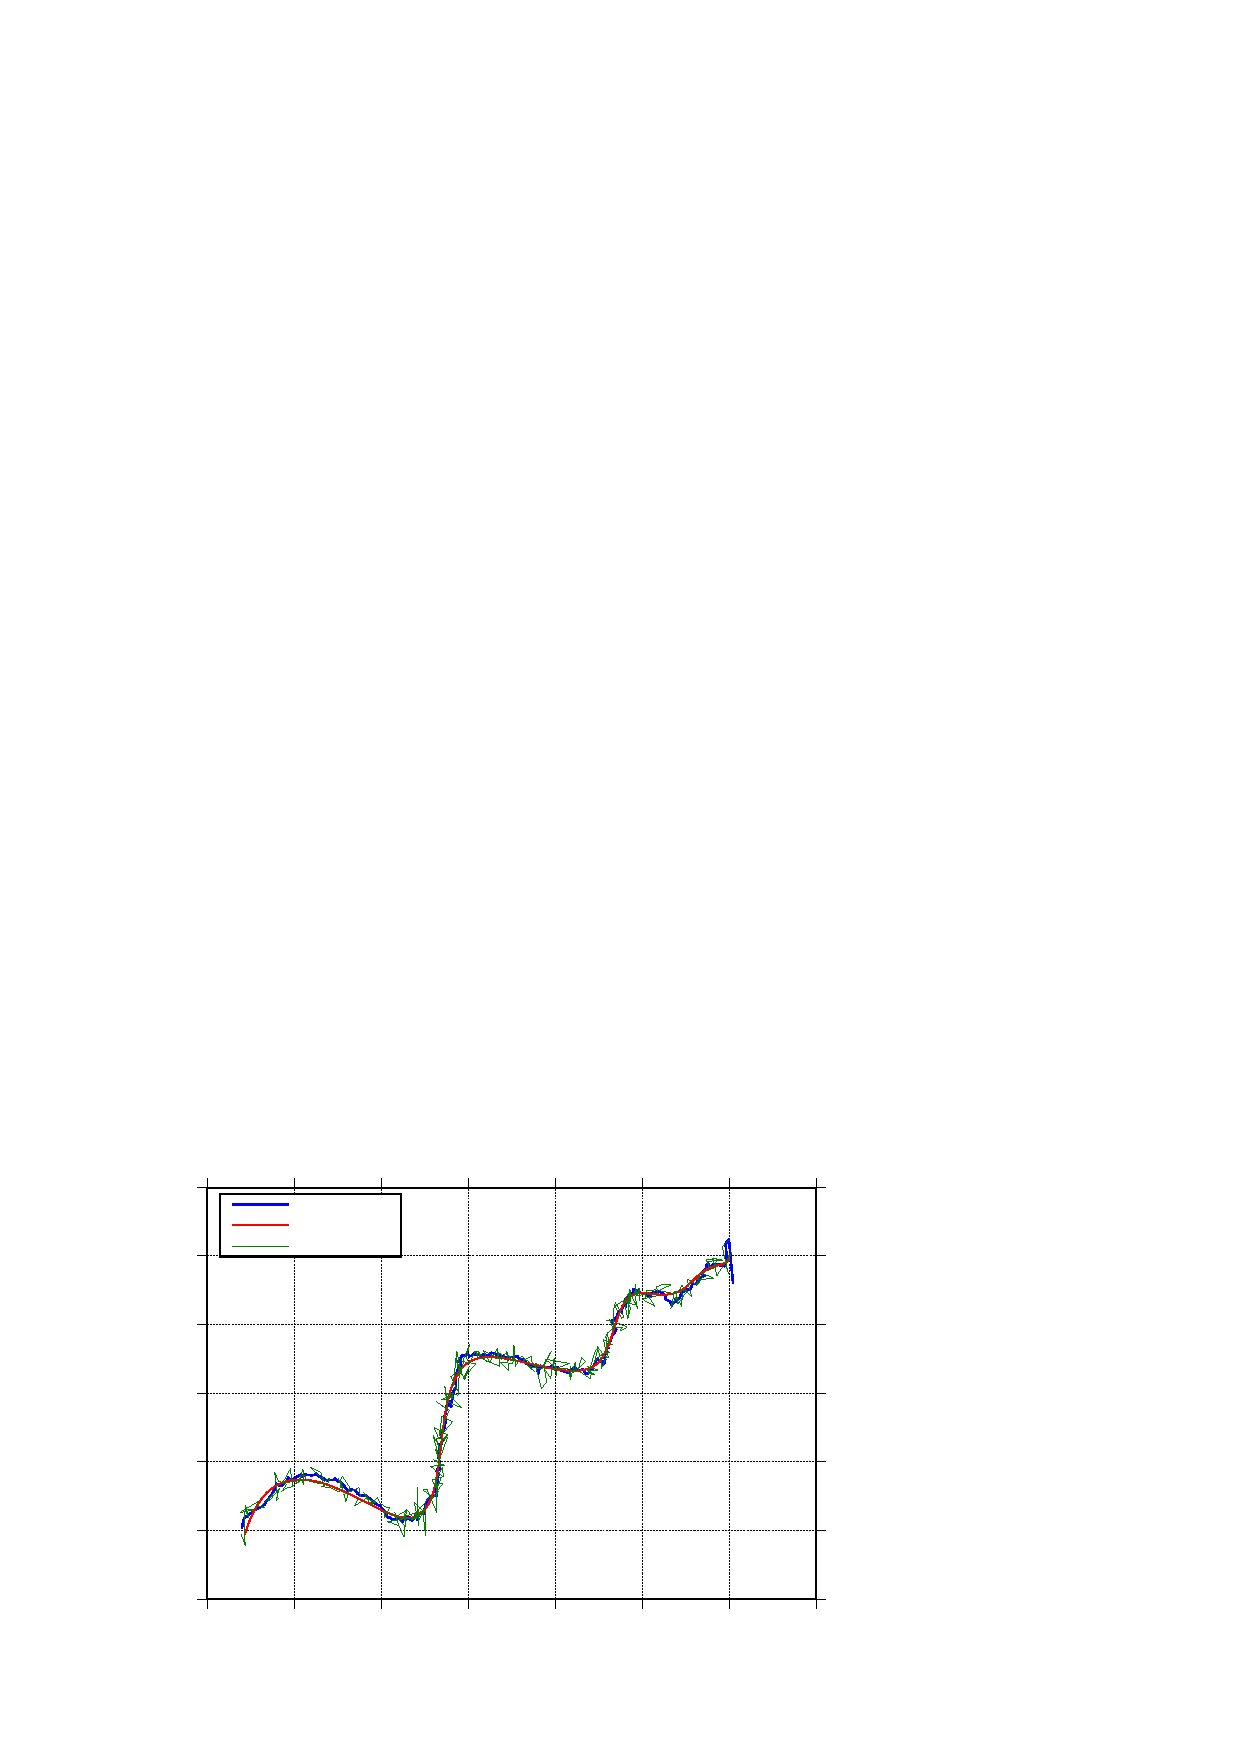
\includegraphics[width=1.0\textwidth,keepaspectratio]{Figuras/graf_ej3a.pdf}
			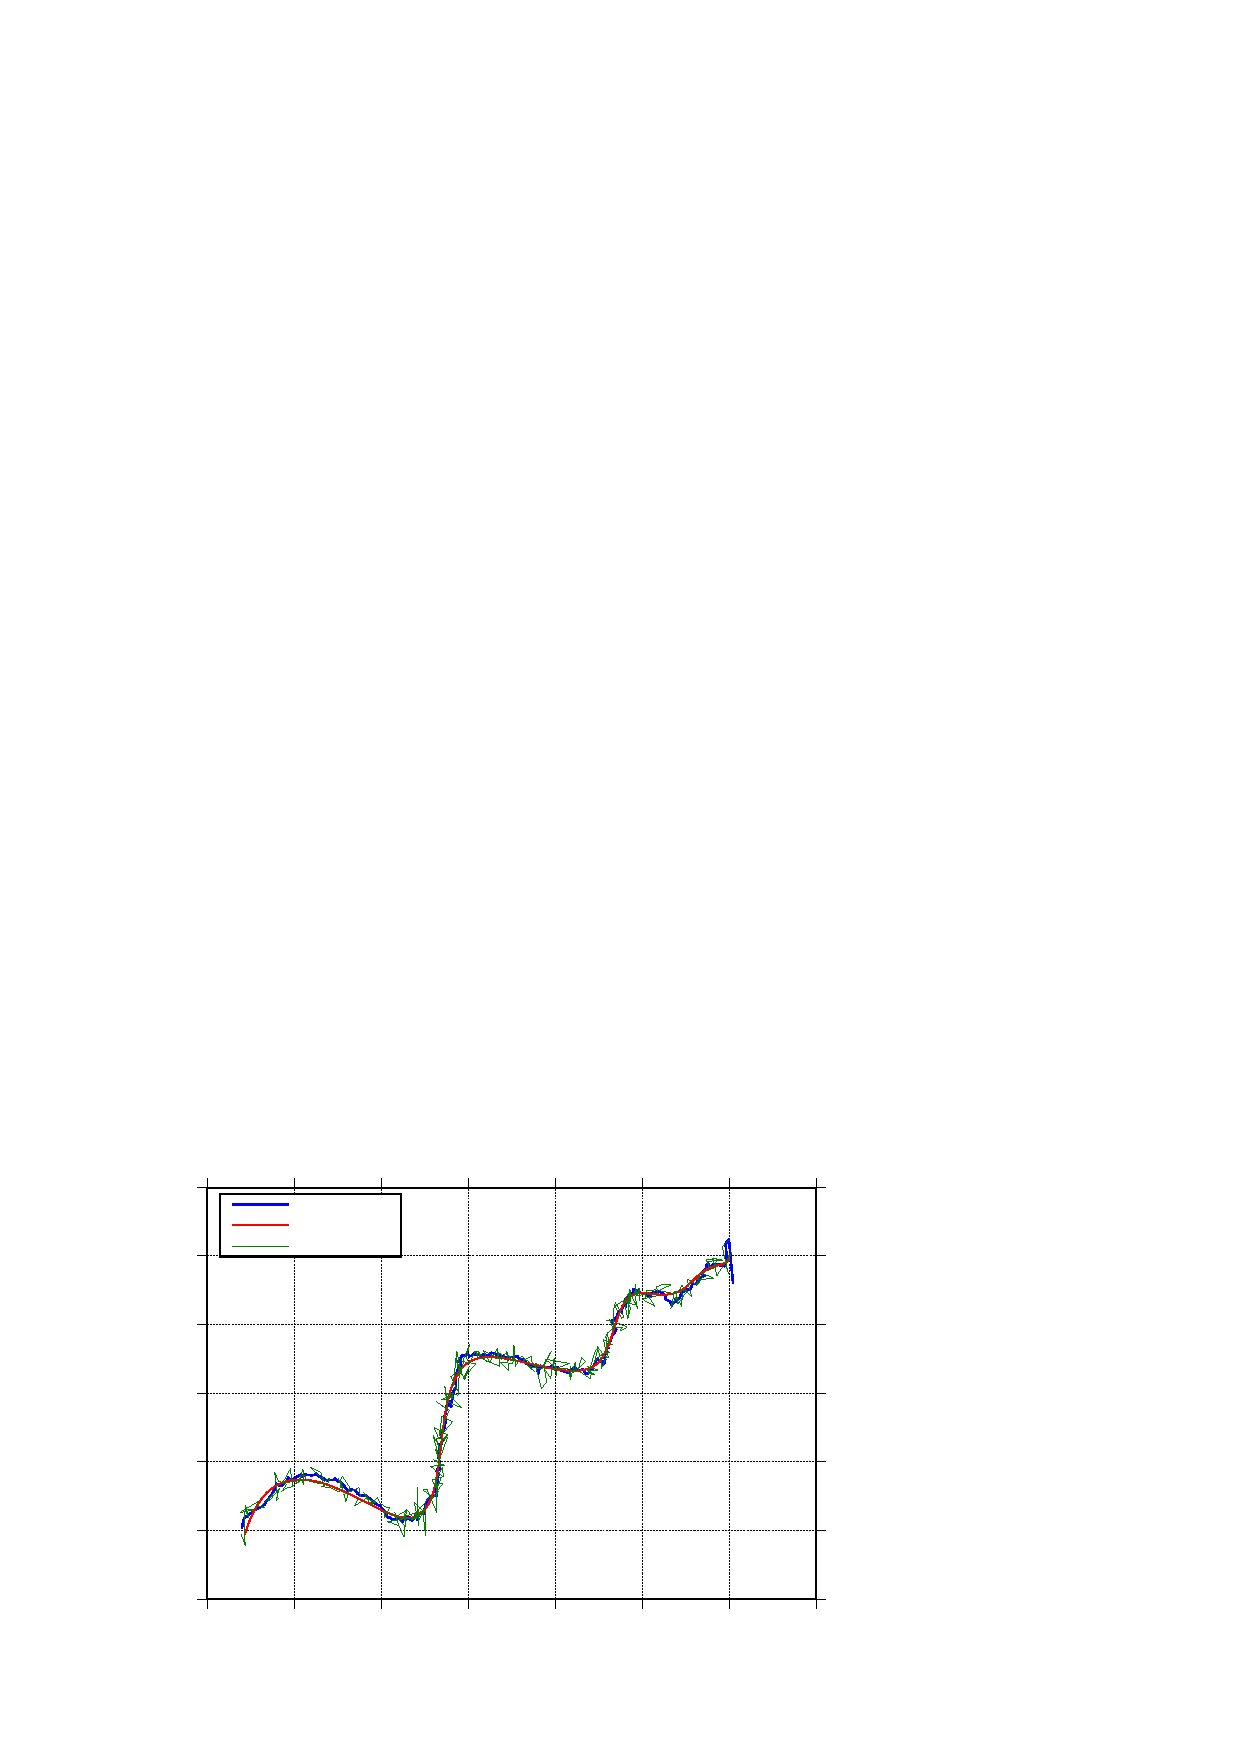
\includegraphics[scale=0.5,trim={6,5cm 0 0 0}]{Figuras/graf_ej3a.pdf}
			\caption{Caso 1}
			\label{fig:ej3a}
		\end{figure}
	
	\subsection{Caso 2 - $\vect{x}_{0/0} = [200\;-3000\;0\;0\;0\;0]^T$, $P^{'}_{0/0}=100\; P_{0|0}$} \label{sec:ej3b}
	
	Ahora se tiene un error en el estado inicial grande, pero al ser la varianza grande el algoritmo sabe que se trata de un valor poco confiable, y no tarda demasiado en corregir la estimación de la trayectoria. El resultado puede verse en la Figura \ref{fig:ej3b}.
		
		\begin{figure}[H]
			\centering
			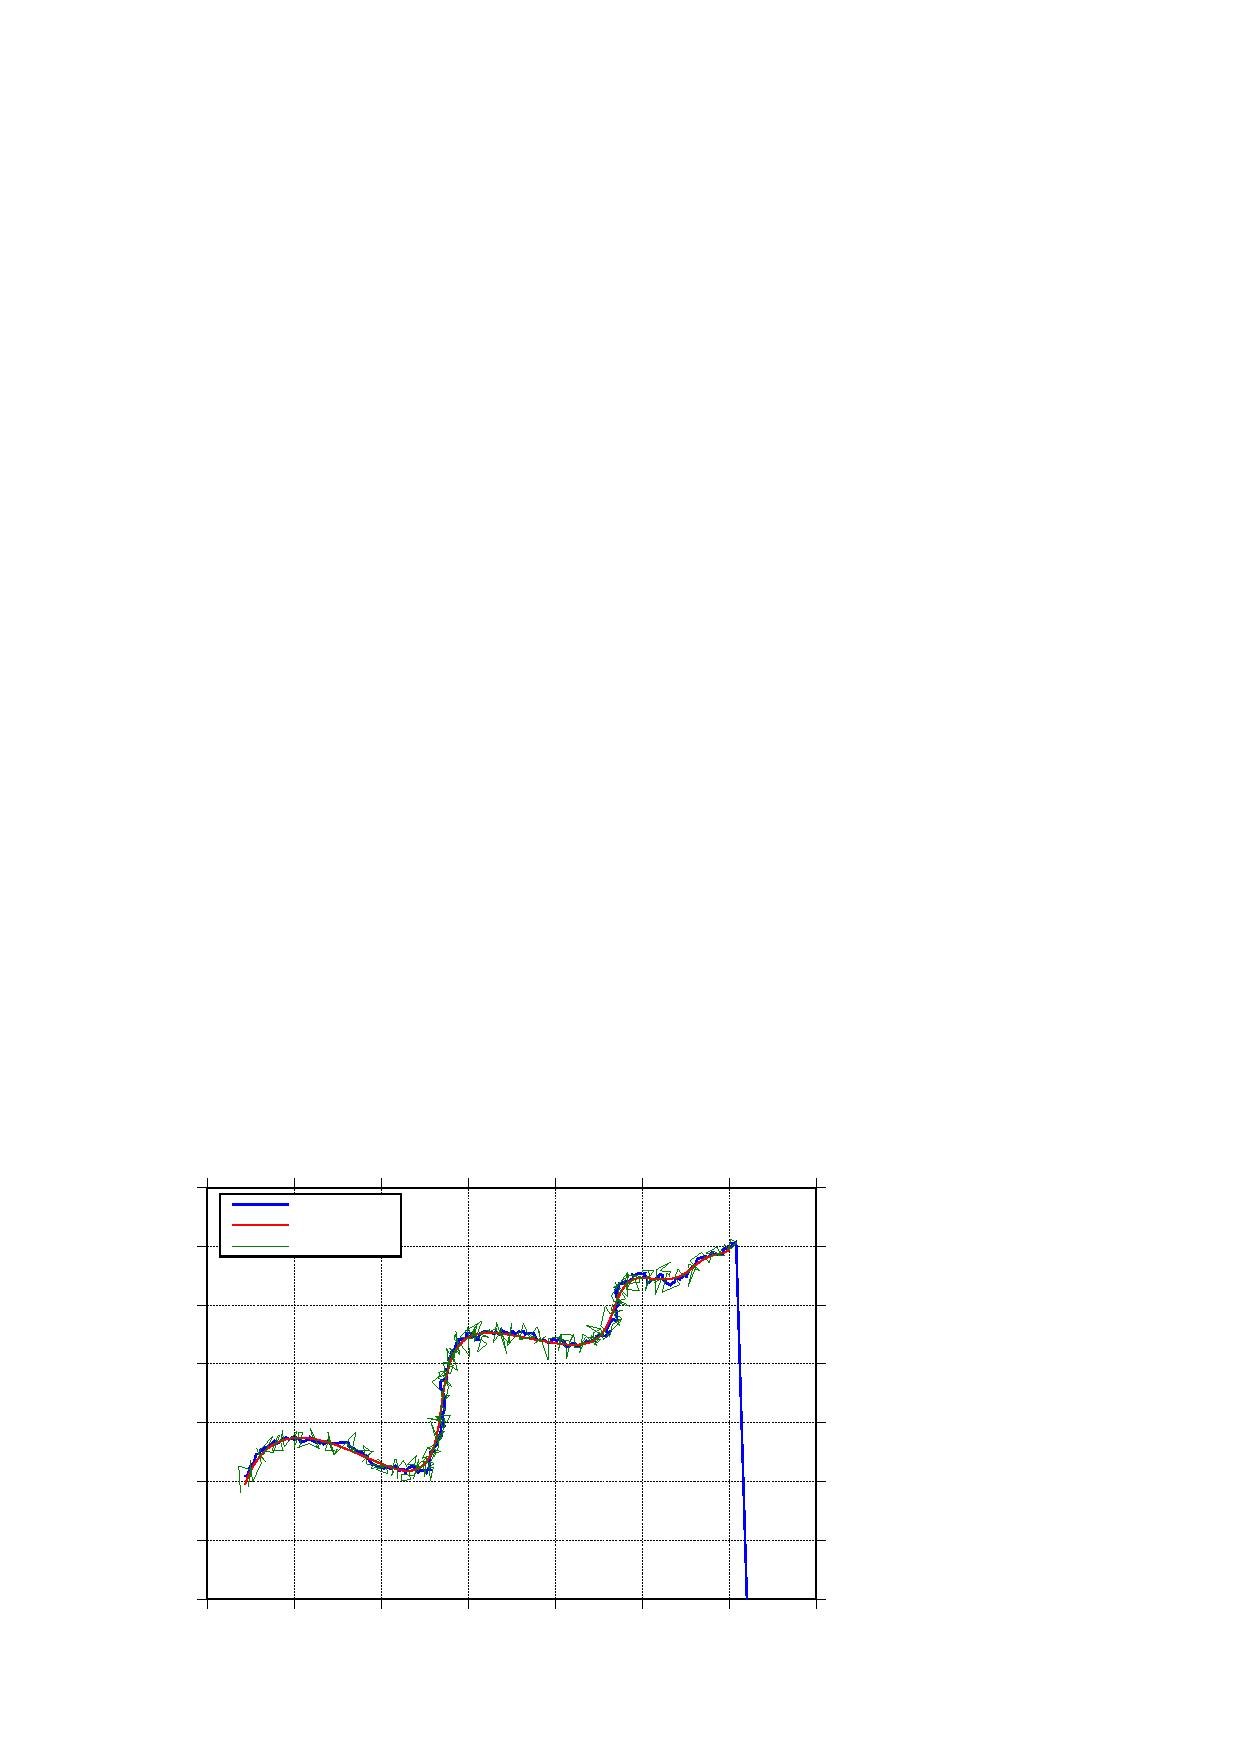
\includegraphics[scale=0.5,trim={6,5cm 0 0 0}]{Figuras/graf_ej3b.pdf}
			\caption{Caso 2}
			\label{fig:ej3b}
		\end{figure}
	\indent Se observa que a comparación a \ref{sec:ej3a}, teniendo una covarianza grande en ambos, el algorítmo converge más rápido con posición inicial más distante del valor real. Al tener un valor inicial más cercano al verdadero, la correlación de las mediciones con dicho valor es menor implicando en innovaciones con menor varianza. Como $P$ es grande, el algoritmo de Kalman genera una ganancia $K$ grande causando que los valores de $\vect{x}_{k/k}$ sigan más a la innovación (medición) que a la predicción a través de la dinámica. En consecuencia, con $P$ grande el algoritmo converge más rápido si el valor inicial no se asemeja al valor verdadero para que las innovaciones provean más información.
	
	\subsection{Caso 3 - $\vect{x}_{0/0} = [40\;-200\;0\;0\;0\;0]^T$, $P^{'}_{0/0}=\num{0.01}\; P_{0|0}$} \label{sec:ej3c}
	
	En este tercer caso el error de la estimacion del estado inicial es pequeño, pero a diferencia del primer caso la varianza es grande. Dado ésto, el algoritmo se confia menos del valor inicial y tarda más en converger que en el primer caso (convergencia del error en \SI{100}{\s} versus \SI{60}{\s}). El resultado puede verse en la Figura \ref{fig:ej3c}.
	
		\begin{figure}[H]
			\centering
			\includegraphics[scale=0.5,trim={6,5cm 0 0 0}]{Figuras/graf_ej3c.pdf}
			\caption{Caso 3}
			\label{fig:ej3c}
		\end{figure}
	
	\subsection{Caso 4 - $\vect{x}_{0/0} = [200\;-30000\;0\;0\;0\;0]^T$, $P^{'}_{0/0}=\num{0.01}\; P_{0|0}$} \label{sec:ej3d}
	
	Finalmente cuando se trata de un error en el estado inicial grande con una varianza pequeña, se ve que es el peor caso. Se está inicializando el algoritmo con un estado incorrecto y además se le está informando que es muy confiable. En el algoritmo en sí se puede ver que con $P$ bajo, se desprecia el aporte de las innovaciones siguiendo la dinámica a partir del valor inicial. Sin embargo, al distar mucho del verdadero, la trayectoria estimada tarda mucho en estabilizarse con respecto a la real (se ve que sigue oscilando para tiempos mayores a \SI{100}{\s}). El resultado puede verse en la Figura \ref{fig:ej3d}.
	
		\begin{figure}[H]
			\centering
			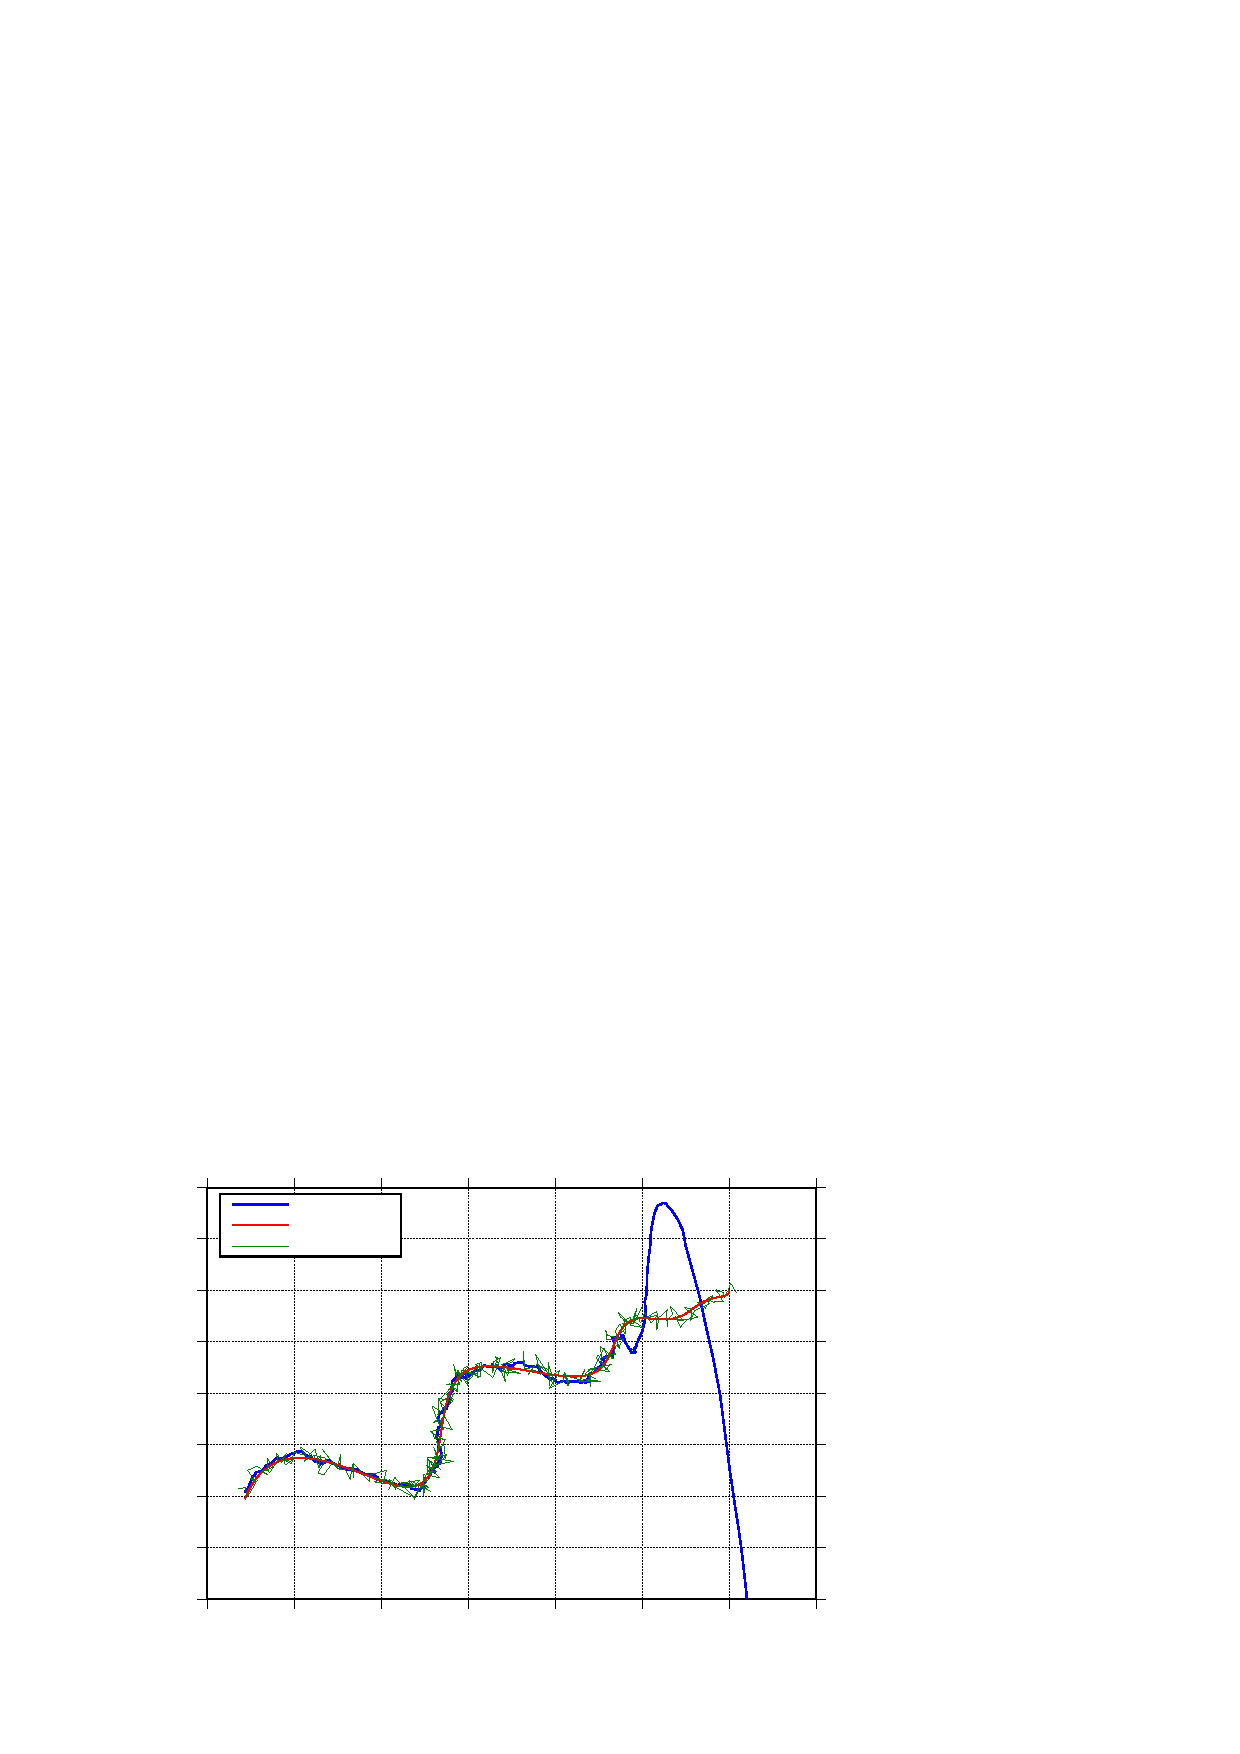
\includegraphics[scale=0.5,trim={6,5cm 0 0 0}]{Figuras/graf_ej3d.pdf}
			\caption{Caso 4}
			\label{fig:ej3d}
		\end{figure}
		
%	\subsection{Script}
%	
%		A continuación presentamos el script de esta sección. Básicamente realiza lo mismo que el punto anterior pero para distintas condiciones iniciales.
%
%	\lstinputlisting[]{EJ3.m}
	


	\section{Ejercicio 4}\label{sec:ej4}
		\subsection{Fundamentos}

	Cuando se trabaja con sensores con ruido de media desconocida, no nula y constante, se propone el siguiente modelo:

	\begin{equation*}
		\vect{\eta}_{n} = \vect{\tilde{\eta}}_{n} + \vect{\mu}
	\end{equation*}

	\begin{equation*}
		\Sigma_{d}:
		\begin{cases}
			\vect{x}_{n + 1} = A_{d}\: \vect{x}_{n} + B_{d} \: \vect{\xi}_{n} \\
			\vect{y}_{n} = C_{d}\: \vect{x}_{n} + \vect{\tilde{\eta}}_{n} + \vect{\mu}
		\end{cases}
	\end{equation*}
	donde ahora el nuevo ruido $\vect{\tilde{\eta}}_{n}$ es de media nula, y se representa la media del ruido como $\vect{\mu}$. Una técnica para llevar el nuevo modelo a la forma del modelo anterior consiste en considerar la media del ruido como un estado más a estimar. De esta forma se incluye dentro de las variables de estado:

	\begin{equation*}
		\vect{z}_{n} = \begin{bmatrix} \vect{x}_{n} \\[0.3em] \vect{\mu}\end{bmatrix} \qquad%
	\end{equation*}
	resultando en:
	
	\begin{equation*}
		\tilde{\Sigma_{d}}:
		\begin{cases}
			\vect{z}_{n + 1} = \tilde{A_{d}}\: \vect{z}_{n} + \tilde{B_{d}} \: \vect{\xi}_{n} \\
			\vect{y}_{n} = \tilde{C_{d}}\: \vect{z}_{n} + \vect{\tilde{\eta}}_{n}
		\end{cases}
	\end{equation*}

	Con las nuevas matrices:
	
	\begin{equation*}
			\tilde{A_{d}} = \begin{bmatrix} A_{d} & 0 \\[0.3em] 0 & I \end{bmatrix}
	\end{equation*}
	
	\begin{equation*}
			\tilde{B_{d}} = \begin{bmatrix} B_{d} \\[0.3em] 0 \end{bmatrix}
	\end{equation*}
	
	\begin{equation*}
			\tilde{C_{d}} = \begin{bmatrix} C_{d} & I \end{bmatrix}
	\end{equation*}
	
	Cabe aclarar que el éxito de esta solución dependerá de la observabilidad del nuevo sistema. A continuación se expondrán las distintas variantes que pueden darse en cuanto a la observabilidad.

%--------------------------------------------------------------------------------------------------

\subsection{Medición de P - Sesgo en P}

	En la Figura \ref{fig:ej4a} se observa el resultado de medir sólo posición, con un sesgo en la misma. En el gráfico, sin la estimación del sesgo, la estimación de la trayectoria se encuentra desviada de la real, de la misma manera que lo están las mediciones. Sin embargo, como en este caso el sesgo no es observable, el resultado estimando con o sin sesgo es el mismo.

	\begin{figure}[H]
		\centering
		%\includegraphics[width=1.0\textwidth,keepaspectratio]{Figuras/graf_ej4a.pdf}
		\includegraphics[scale=0.5,trim={6,5cm 0 0 0}]{Figuras/graf_ej4a.pdf}
		\caption{Estimación De Trayectoria}
		\label{fig:ej4a}
	\end{figure}
	
	En la Figura \ref{fig:ej4a_bias} se observa la convergencia de la estimación del sesgo. Es posible ver que no converge exactamente al valor deseado ($\vect{b}_p = [\SI{300}{\m}\; \SI{200}{\m}]^T$).
	
	\begin{figure}[H]
		\centering
		\includegraphics[width=0.7\textwidth,keepaspectratio]{Figuras/bias_ej4a.pdf}
		\caption{Estimación Del Sesgo}
		\label{fig:ej4a_bias}
	\end{figure}
	
	En la Figura \ref{fig:ej4a_cov} se observa la autocorrelación de las innovaciónes. Es posible ver que se trata de un proceso blanco.
	
	\begin{figure}[H]
		\centering
		\includegraphics[width=1.0\textwidth,keepaspectratio]{Figuras/covinn_ej4a.pdf}
		\caption{Correlación De Innovaciones}
		\label{fig:ej4a_cov}
	\end{figure}
	
%--------------------------------------------------------------------------------------------------

\subsection{Medición de PVA - Sesgo en P}

	En la Figura \ref{fig:ej4b} se observa el resultado de la estimación de la trayectoria. Éste resulta similar al caso anterior, dado que tampoco se tiene observabilidad en el sesgo.

	\begin{figure}[H]
		\centering
		\includegraphics[scale=0.5,trim={6,5cm 0 0 0}]{Figuras/graf_ej4b.pdf}
		\caption{Estimación De Trayectoria}
		\label{fig:ej4b}
	\end{figure}
	
	En la Figura \ref{fig:ej4b_bias} se observa la convergencia de la estimación del sesgo. Es posible ver que no converge exactamente al valor deseado, al igual que en el caso anterior.
	
	\begin{figure}[H]
		\centering
		\includegraphics[width=0.7\textwidth,keepaspectratio]{Figuras/bias_ej4b.pdf}
		\caption{Estimación Del Sesgo}
		\label{fig:ej4b_bias}
	\end{figure}
	
	En la Figura \ref{fig:ej4b_cov} se observa la autocorrelación de las innovaciónes. Es posible ver que se trata de un proceso blanco.
	
	\begin{figure}[H]
		\centering
		\includegraphics[width=1.0\textwidth,keepaspectratio]{Figuras/covinn_ej4b.pdf}
		\caption{Correlación De Innovaciones}
		\label{fig:ej4b_cov}
	\end{figure}
	
%--------------------------------------------------------------------------------------------------
	
\subsection{Medición de V - Sesgo en V}

	En la Figura \ref{fig:ej4c} se observa el resultado de la estimación. En la misma la estimación no sólo no sigue la trayectoria, sino que se aparta cada vez más de ella a medida que transcurre el tiempo, tanto si se ignora el sesgo, como si se trata de estimarlo (problemas de observabilidad).

	\begin{figure}[H]
		\centering
		\includegraphics[scale=0.5,trim={6,5cm 0 0 0}]{Figuras/graf_ej4c.pdf}
		\caption{Estimación De Trayectoria}
		\label{fig:ej4c}
	\end{figure}
	
	En la Figura \ref{fig:ej4c_bias} se observa que la estimación del sesgo converge, pero no a los valores correctos como es de esperar.
	
	\begin{figure}[H]
		\centering
		\includegraphics[width=0.7\textwidth,keepaspectratio]{Figuras/bias_ej4c.pdf}
		\caption{Estimación Del Sesgo}
		\label{fig:ej4c_bias}
	\end{figure}
	
	En la Figura \ref{fig:ej4c_cov} se observa la autocorrelación innovaciónes. Es posible ver que el proceso ya no es del todo blanco.
	
	\begin{figure}[H]
		\centering
		\includegraphics[width=1.0\textwidth,keepaspectratio]{Figuras/covinn_ej4c.pdf}
		\caption{Correlación De Innovaciones}
		\label{fig:ej4c_cov}
	\end{figure}
	
%--------------------------------------------------------------------------------------------------

\subsection{Medición de PVA - Sesgo en V}

	En la Figura \ref{fig:ej4d} puede observarse el resultado de la estimación. En este caso no se tienen problemas de observabilidad, por lo que la estimación sigue la trayectoria y además sigue los valores de velocidad reales.

	\begin{figure}[H]
		\centering
		\includegraphics[scale=0.5,trim={6,5cm 0 0 0}]{Figuras/graf_ej4d.pdf}
		\caption{Estimación De Trayectoria}
		\label{fig:ej4d}
	\end{figure}
	
	En la Figura \ref{fig:ej4d_bias} se observa la convergencia de la estimación del sesgo. Al no tener problemas de observabilidad, puede comprobarse que converge a los valores correctos ($\vect{b}_v = [\SI{10}{\m\per\s} \; \SI{20}{\m\per\s}]^T$).
	
	\begin{figure}[H]
		\centering
		\includegraphics[width=0.7\textwidth,keepaspectratio]{Figuras/bias_ej4d.pdf}
		\caption{Estimación Del Sesgo}
		\label{fig:ej4d_bias}
	\end{figure}
	
	En la Figura \ref{fig:ej4d_cov} se observa la autocorrelación de las innovaciones. Allí puede notarse que ya no es un proceso blanco, a pesar de que se estiman bien los estados.
	
	\begin{figure}[H]
		\centering
		\includegraphics[width=1.0\textwidth,keepaspectratio]{Figuras/covinn_ej4d.pdf}
		\caption{Correlación De Innovaciones}
		\label{fig:ej4d_cov}
	\end{figure}

%--------------------------------------------------------------------------------------------------

\subsection{Medición de A - Sesgo en A}

	En la Figura \ref{fig:ej4e} podemos observar el resultado de la estimación. En este caso no se tiene observabilidad, por lo que el resultado empeora cada vez más a medida que pasa el tiempo.

	\begin{figure}[H]
		\centering
		\includegraphics[scale=0.5,trim={6,5cm 0 0 0}]{Figuras/graf_ej4e.pdf}
		\caption{Estimación De Trayectoria}
		\label{fig:ej4e}
	\end{figure}
	
	En la Figura \ref{fig:ej4e_bias} podemos observar la convergencia de la estimación. Si bien la misma converge, al no tener observabilidad no lo hace a los valores correctos.
	
	\begin{figure}[H]
		\centering
		\includegraphics[width=0.7\textwidth,keepaspectratio]{Figuras/bias_ej4e.pdf}
		\caption{Estimación Del Sesgo}
		\label{fig:ej4e_bias}
	\end{figure}
	
	En la Figura \ref{fig:ej4e_cov} observamos la autocorrelación de las innovaciones. Puede verse que no se trata de un proceso totalmente blanco.
	
	\begin{figure}[H]
		\centering
		\includegraphics[width=1.0\textwidth,keepaspectratio]{Figuras/covinn_ej4e.pdf}
		\caption{Correlación De Innovaciones}
		\label{fig:ej4e_cov}
	\end{figure}

%--------------------------------------------------------------------------------------------------

\subsection{Medición de PVA - Sesgo en A}

	En la Figura \ref{fig:ej3f} se observa el resultado de la estimación. Nuevamente no se tienen problemas de observabilidad, por lo que la estimación sigue la trayectoria y, además, sigue la aceleración de forma correcta.

	\begin{figure}[H]
		\centering
		\includegraphics[scale=0.5,trim={6,5cm 0 0 0}]{Figuras/graf_ej4f.pdf}
		\caption{Estimación De Trayectoria}
		\label{fig:ej3f}
	\end{figure}
	
	En la Figura \ref{fig:ej3f_bias} se observa la convergencia de la estimación del sesgo. Al tener observabilidad, puede comprobarse que converge a los valores correctos ($\vect{b}_a = [\SI{1}{\m\per\s\squared} \; \SI{2}{\m\per\s\squared}]^T$).
	
	\begin{figure}[H]
		\centering
		\includegraphics[width=0.7\textwidth,keepaspectratio]{Figuras/bias_ej4f.pdf}
		\caption{Estimación Del Sesgo}
		\label{fig:ej3f_bias}
	\end{figure}
	
	En la Figura \ref{fig:ej3f_cov} se observa la autocorrelación de las innovaciones. Puede verse que no se trata de un proceso blanco.

	\begin{figure}[H]
		\centering
		\includegraphics[width=1.0\textwidth,keepaspectratio]{Figuras/covinn_ej4f.pdf}
		\caption{Correlación De Innovaciones}
		\label{fig:ej3f_cov}
	\end{figure}
	
%--------------------------------------------------------------------------------------------------

	\subsection{Test de observabilidad}

	Al realizar el test de observabilidad a los 6 casos anteriores se obtiene la siguiente tabla que lo resume:

		\begin{table}[h!]
			\centering
			\begin{tabular}{cccc}
				\toprule
				Medición	& Sesgo		& Cantidad no observables	& Observables\\
				\midrule
				$\vect{p}$	& $\vect{b}_p$	& 2				& $\vect{p}$ $\vect{v}$ $\vect{a}$\\
				$\vect{p}$ $\vect{v}$ $\vect{a}$	& $\vect{b}_p$	& 2				& $\vect{p}$ $\vect{v}$ $\vect{a}$\\
				$\vect{v}$	& $\vect{b}_v$	& 4				& $\vect{v}$ $\vect{a}$ \\
			$\vect{p}$ $\vect{v}$ $\vect{a}$	& $\vect{b}_v$	& 0				& $\vect{p}$ $\vect{v}$ $\vect{a}$ $\vect{b}_v$ \\
				$\vect{a}$	& $\vect{b}_a$	& 6				& $\vect{a}$\\
			$\vect{p}$ $\vect{v}$ $\vect{a}$	& $\vect{b}_a$	& 0				& $\vect{p}$ $\vect{v}$ $\vect{a}$ $\vect{b}_a$ \\

				\bottomrule
			\end{tabular}
				\caption{Test de observabilidad para el ejercicio 4.}
				\label{tab:obs_ej2}
		\end{table}



\subsection{Script}

A continuación se incluye el script que realiza la estimación. Puede seleccionarse mediante las variables \texttt{bool\_p}, \texttt{bool\_v}, \texttt{bool\_a}, en 1 o en 0, qué se va a medir. Por otro lado puede seleccionarse mediante las variables \texttt{bool\_pb}, \texttt{bool\_vb}, \texttt{bool\_ab}, en 1 o en 0, en qué variables se desea tener sesgo.
	
	\lstinputlisting[firstline=20, firstnumber=20, lastline=28]{EJ4a.m}
	\lstinputlisting[firstline=130, firstnumber=130, lastline=180]{EJ4a.m}

%--------------------------------------------------------------------------------------------------


	\section{Conclusiones}\label{sec:conclusiones}
		\begin{itemize}  
\item La importancia del trabajo se centra en entender el funcionamiento general del circuito, a partir de ser descompuesto en distintos bloques	



\item The second item 



\item The third etc \ldots 



\end{itemize}


	% \appendix
\end{document}
